\section{Optix: движок трассировки лучами общего назначения}
\begin{figure}[h]
\center{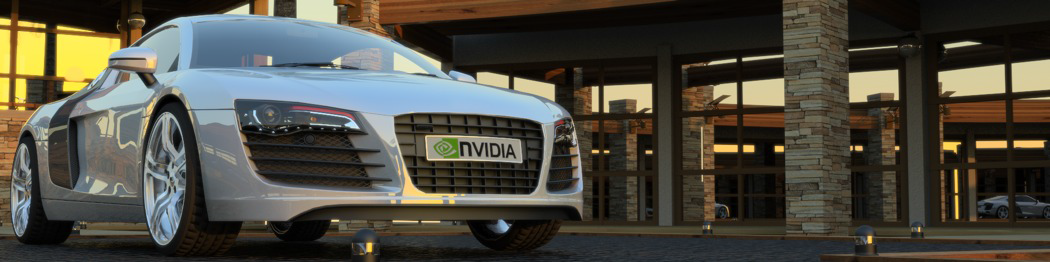
\includegraphics[width=1\linewidth]{audi.png}}
\caption{Изображение из приложения созданого в OptiX.}
\label{audi}
\end{figure}
\subsection{Краткий обзор}
Механизм трассировки лучей NVIDIA® OptiX™ --- программируемая система, разработанная для графических ускорителей NVIDIA и других массивно-параллельных архитектур.
Механизм OptiX основывается на базовом наблюдении, что большинство алгоритмов трассировки лучей могут быть реализованы, используя маленький набор программируемых операций. 
Следовательно, ядро OptiX --- проблемно-ориентированный JIT компилятор, который генерирует пользовательские ядра трассировки лучей, комбинируя предоставленные пользователями программы для генерации луча, заливки материала, объектного пересечения и обхода сцены. 
Оно включает реализацию очень широкого набора основанных на трассировке лучей алгоритмов и приложений, включая интерактивный рендеринг, оффлайн рендеринг, системы обнаружения коллизий, запросы искусственного интеллекта и научного моделирования, такие как звуковое распространение. 
OptiX достигает высокой производительности через компактную объектную модель и применения нескольких специфичной для трассировки лучей оптимизаций компилятора. 
Для простоты использования OptiX представляет модель программирования единственного луча с полной поддержкой рекурсии и динамического механизма отправки, подобного вызовам виртуальной функции.

\subsection{Введение}
Чтобы решить проблему создания доступной, гибкой, и эффективной системы трассировки лучей для массивно-параллельной архитектуры, представляем OptiX --- механизм трассировки лучей общего назначения. 
Этот механизм комбинирует программируемый конвейер трассировки лучей с легким представлением сцены. 
Общий интерфейс программирования включает реализацию множества основанных на трассировке лучей алгоритмов в графических и неграфических доменах, таких как рендеринг, звуковое распространение, обнаружение коллизий и искусственный интеллект.

В этом разделе мы обсуждаем цели проекта OptiX, а также реализации для NVIDIA Quadro®, GeForce® и Tesla® GPUs. 
Мы рассмотрим проблемно-ориентированную компиляцию с гибким набором средств управления иерархией сцены, ускоряющего создания структуры и обхода, непрерывного обновления сцены и динамично сбалансированной с загрузки модели выполнения GPU. 

Чтобы создать систему для широкого диапазона задач трассировки лучей, были принято несколько компромиссов и проектных решений, которые привели к следующим особенностям:
\begin{itemize}
 \item Общий низкоуровневый механизм трассировки лучей. 
 Механизм OptiX фокусируется исключительно на фундаментальных вычислениях, требуемых для трассировки лучей, и избегает встраивания конструкции для рендеринга. 
 Движок представляет механизмы для выражения взаимодействий геометрии луча и не имеет встроенного понятия световых сигналов, теней, коэффициента отражения, и т.д.

\item Программируемый конвейер трассировки лучей. 
Механизм OptiX демонстрирует, что большинство алгоритмов трассировки лучей может быть реализовано, используя маленький набор легких программируемых операций. 
Это определяет абстрактную модель выполнения трассировки лучей, поскольку последовательность пользователя определила программы. 
Эта модель при объединении с произвольными данными, хранившимися с каждым лучом, может использоваться, чтобы реализовать множество сложных графических сцен и невизуальных алгоритмов.

\item Простая модель программирования. 
Механизм OptiX обеспечивает такие механизмы выполнения, что программисты пользуются знакомыми методами работы с трассировкой лучами и  не обременяют себя низкоуровневой оптимизацией. 
Движок представляет знакомую рекурсивную, модель программирования единственного луча, а не пакеты луча или явные конструкции SIMD-стиля. 

\item Проблемно-ориентированный компилятор. 
Механизм OptiX комбинирует своевременные методы компиляции со специфичным для трассировки лучей знанием, чтобы реализовать его модель программирования эффективно. 
Абстракция механизма разрешает компилятору настраивать модель выполнения для доступных системных аппаратных средств.

\item Эффективное представление сцены. 
Механизм OptiX реализует объектную модель, которая использует динамическое наследование, чтобы упростить компактное представление параметров сцены. 
Гибкая система графика узла позволяет сцене быть организованной для максимальной производительности, все еще поддерживая инстанцирование, многоуровневую детализацию и вложенные ускоряющие структуры.

\end{itemize}


\subsection{Программируемый конвейер трассировки лучей}
Центральная идея механизма OptiX состоит в том, что большинство алгоритмов трассировки лучей может быть реализовано, используя маленький набор программируемых операций. 
Это прямой аналог к программируемым конвейерам растеризации, используемым OpenGL и Direct3D. 
На высоком уровне те системы представляют абстрактный растеризатор, содержащий легкие обратные вызовы для штриховки вершины, обработки геометрии, составления мозаики и операций штриховки фрагмента. 
Ансамбль этих типов программ, обычно используемых в многократных передачах, может использоваться, чтобы реализовать широкий спектр основанных на растеризации алгоритмов. 
 
Мы идентифицировали соответствующее абстрактное выполнение трассировки лучей модель вместе с легкими операциями, которые могут быть настроены реализовывать большое разнообразие основанных на трассировке лучей алгоритмов.[NVIDIA 2010a]. 
Эти операции или программы, могут быть объединенны с определяемой пользователем структурой данных (payload), связанной с каждым лучом. 
Ансамбль программ действует сообща для реализации алгоритма определенного клиентского приложения.

\subsubsection{Программы}
Есть семь различных типов программ в OptiX, каждая из которых работает над одним лучом одновременно.
Кроме того, программа ограничительной рамки действует на геометрию, чтобы определить границы примитива для построения ускоряющей структуры.
Сочетание пользовательских программ и жестко закодированного OptiX ядра образует конвейер трассировки лучей, который описан на рисунке~\ref{fig:graph-of-calling}. 
В отличие от конвейера прямой подачи растеризации более естественно думать о конвейере трассировки лучей как о графе вызовов.
Основная операция, rtTrace, чередуется между поиском пересечения (Traverse) и реагированием на этой пересечение (Shade).
При записи или чтении данных в объявленном пользователем payload луча и в массивах глобальной памяти устройства (буферы), эти операции объединяются для выполнения произвольных вычислений во время трассировки лучей.

Программы генерации лучей являются начальной точкой в конвейере трассировки лучей.
Один вызов rtContextLaunch создаст много экземпляров этих программ.
В примере на рисунке 3 программа генерации луча создает луч с использованием модели камеры pinhole для одного пикселя, начинает операцию трассировки и сохраняет результирующий цвет в выходной буфер.
 С помощью этого механизма, можно также выполнять другие операции, такие как создание фотонных карт, вычисления освещения методом отжига, обработки запросов лучей, переданных из OpenGL, стрельба несколькими лучами для суперсемплинга или реализации различных моделей камер.
Программы пересечения реализуют тесты пересечения лучевой геометрии.
При пересечении ускоряющих структур система будет вызывать программу пересечения, чтобы выполнить геометрический запрос.
Программа определяет, и где луч касается объекта и может вычислять нормали, текстурных координат, или другие атрибуты в зависимости от положения попадания.
Произвольное количество атрибутов могут быть связаны с каждым пересечением.
Программы пересечения включают поддержку произвольных поверхностей, таких как сферы, цилиндры, поверхностей высокого порядка, или даже фрактальной геометрии, как множество Жюлиа.
Тем не менее, даже в системах,состоящих только из треугольников, можно встретить большое разнообразие представлений сетки.
Программируемая операция пересечения облегчает прямой доступ в оригинальном формате, который может помочь избежать копии при взаимодействии с системами на основе растеризации.
\begin{figure}[h]
\center{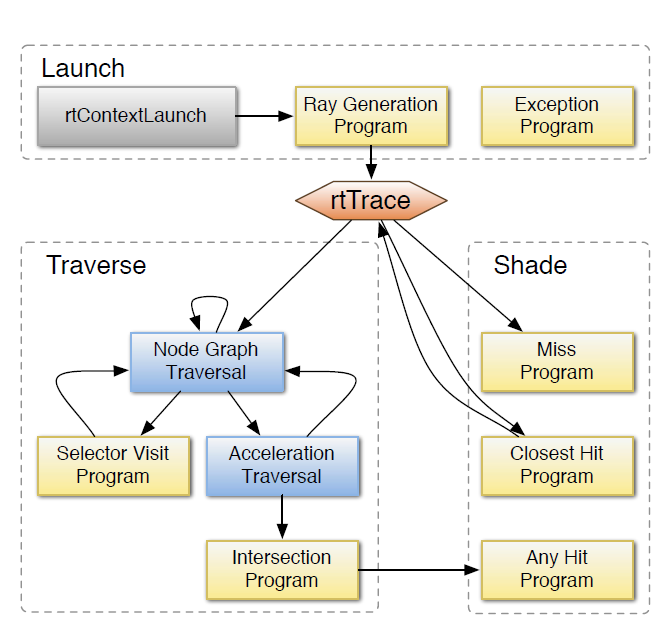
\includegraphics[width=0.7\linewidth]{fig.png}}
\captionГраф вызова, показывающий поток управления по конвейеру трассировки лучей.Желтые прямоугольники представляют указанные пользователем программы, а синие прямоугольники ---алгоритмы внутренние для OptiX.
Выполнение инициируется вызовом API rtContextLaunch.Встроенная функция, rtTrace, может быть использована в программе генерации лучей для отправки лучей в сцену.
Эта функция также может вызываться рекурсивно программой ближайшего попадания для тени и вторичных лучей.
Программа исключения выполняется, когда выполнение отдельного луча завершилось с ошибкой, такой как чрезмерное потребление памяти.}
\label{fig:graph-of-calling}
\end{figure}

Программы ограничительной рамки вычисляют границы, связанные с каждым примитивом для включения ускоряющей структуры над произвольной геометрией.
Учитывая примитивный индекс, простая программа такого типа может, например, читать вершинные данные из буфера и вычислять треугольники ограничительной рамки.
Процедурная геометрия может иногда только оценить границы примитива.
Такие оценки допускаются пока они консервативны, но свободные границы могут привести к снижению производительности.

Ближайшие программы попадания вызываются один раз обхода нашла ближайший  пересечение луча с геометрии сцены.
 Этот тип программы очень напоминает поверхностный шейдеров в классических системах визуализации.
 Как правило, программа ближайшего попадания будет выполнять вычисления, такие как затенение, потенциальное излучение новых лучей в процессе, и сохранение результирующих данных в payload луча.

Любые программы хита вызывают во время обхода для каждого объектного лучом перекрестка, который найден. Любая программа хита позволяет материалу участвовать в объектных решениях перекрестка при разделении операций штриховки от операций геометрии.Это может дополнительно завершить луч, используя встроенную функцию rtTerminateRay, который остановит весь обход и раскрутит стек вызовов к новому вызову rtTrace. Это - легкий механизм исключения, который может использоваться, чтобы реализовать раннее завершение луча для теневых лучей и окружающего поглощения газов. Альтернативно, любая программа хита может проигнорировать перекресток, используя rtIgnoreIntersection, позволяя обходу продолжать искать другие геометрические объекты. Перекресток может быть проигнорирован, например, на основе поиска канала текстуры, таким образом реализовывая эффективную отображенную на альфу прозрачность, не перезапуская обход.
\begin{verbatim}
RT_PROGRAM void pinhole_camera() {
Ray ray = PinholeCamera::makeRay( launchIndex );
UserPayload payload;
rtTrace( topObject, ray, payload );
outputBuffer[launchIndex] = payload.result;
}
\end{verbatim}
ПОДПИСЬ{Программа генерации луча в качестве примера (в CUDA C) для единственной выборки за пиксель. 2-мерное расположение сетки вызов программы дан семантической переменной launchIndex, который используется, чтобы создать основной луч, используя модель камеры с точечной диафрагмой. После трассировки луча вызванные материальные программы хита заполняют поле результата определяемой пользователем структуры полезной нагрузки. Переменная topObject относится к расположению в иерархии сцены, где обход луча должен запуститься, обычно корень графика узла. В
расположение, определенное launchIndex, результат записан в буфер вывода, который будет выведен на экран приложением.}


  Другой вариант использования для любой программы хита может быть найден в Разделе 8.1, где приложение выполняет затухание видимости для частичных теней, брошенных стеклянными объектами. Обратите внимание на то, что перекрестки могут быть представлены не в порядке. Значение по умолчанию, которое любая программа хита не, который часто является желаемой работой.

  Программы мисс выполняются, когда луч не пересекает геометрии в обеспеченном интервале. Они могут использоваться, чтобы реализовать цвет фона или поиск карты среды. Программы исключения выполняются, когда система встречается с исключительным условием, например, когда стек рекурсии превышает объем памяти, доступный для каждого потока, или когда буферный индекс доступа вне диапазона. OptiX также поддерживает определяемые пользователем исключенияэто может быть брошено из любой программы. 
  
  Программа исключения может реагировать, например, распечатывая диагностические сообщения или визуализируя условие при записи специальных значений цвета в буфер выходного пикселя. 

Селекторные программы посещения представляют программируемость для обхода графика узла крупного уровня. Например, приложение может принять решение изменить уровень геометрической детали для частей сцены на perray основе. В этом случае программа посещения исследовала бы луч
расстояние или дифференциал луча, сохраненный полезной нагрузкой и, принимают пересекающееся решение на основе тех данных.
\subsubsection{Представление сцены}
Механизм OptiX использует гибкую структуру для представления информации о сцене и связал программируемые операции, собранный в контейнерном объекте вызывал контекст. Это представление - также механизм для привязки программируемых программ построения теней к объектно-специфичные данные, которых они требуют. В сочетании с объектной моделью специального назначения, описанной в Разделе 3.3, достигнуто компактное представление данных сцены.
\paragraph{Узлы иерархии.}

Сцена представлена как график. Это представление очень легко и управляет обходом лучей через сцену. Это может также использоваться, чтобы реализовать инстанцирующие двухуровневые иерархии для анимаций твердых объектов или другие общие структуры сцены. Чтобы поддерживать инстанцирование и совместное использование общих данных, у узлов могут быть многократные родители.

Четыре основных типов узлов могут использоваться, чтобы обеспечить представление сцены, используя направленный граф. Любой узел может использоваться в качестве корня обхода сцены. Это позволяет, например, различным представлениям использоваться для различных типов луча. 

Узлы группы содержат нуль или больше (но обычно два или больше) дочерние элементы любого типа узла. Узлу группы связали ускоряющую структуру с ним и может использоваться, чтобы обеспечить верхний уровень двухуровневой пересекающейся структуры.

Узлы Geometry Group - листы графика и содержат примитивные и материальные объекты, описанные ниже. Этому типу узла также связали ускоряющую структуру с ним. Любая непустая сцена будет содержать по крайней мере одну группу геометрии.
Преобразуйте узлы, имеют единственный дочерний элемент любого типа узла, плюс связанное $4\times3$ матрица, которая используется, чтобы выполнить аффинное преобразование базовой геометрии.

У селекторных узлов есть нуль или больше дочерних элементов любого типа узла плюс единственная программа посещения, которая выполняется, чтобы выбрать среди доступных дочерних элементов. Несмотря на то, что не реализованный в текущей версии библиотек OptiX, график узла может быть циклическим, если селекторный узел используется тщательно, чтобы избежать бесконечной рекурсии.
\paragraph{ Геометрия и материальные объекты.}

Объем данных сохранен в узлах геометрии в листах графика. Они содержат объекты, которые определяют операции штриховки и геометрия. У них могут также быть многократные родители, позволяя материалу и информации о геометрии быть совместно использованным в многократных точках в графике; для полного примера посмотрите рисунок 4. Объекты Экземпляра геометрии связывают объект геометрии с рядом материальных объектов. Это - общая структура, используемая графиками сцены, чтобы сохранить геометрическую и заштриховывающую информацию ортогональной. Объекты геометрии содержат список геометрических примитивов. Каждый объект геометрии связан с программой ограничивающего прямоугольника и программой перекрестка, оба из которых совместно использованы среди примитивов объекта геометрии.

\begin{figure}[h!]
\center{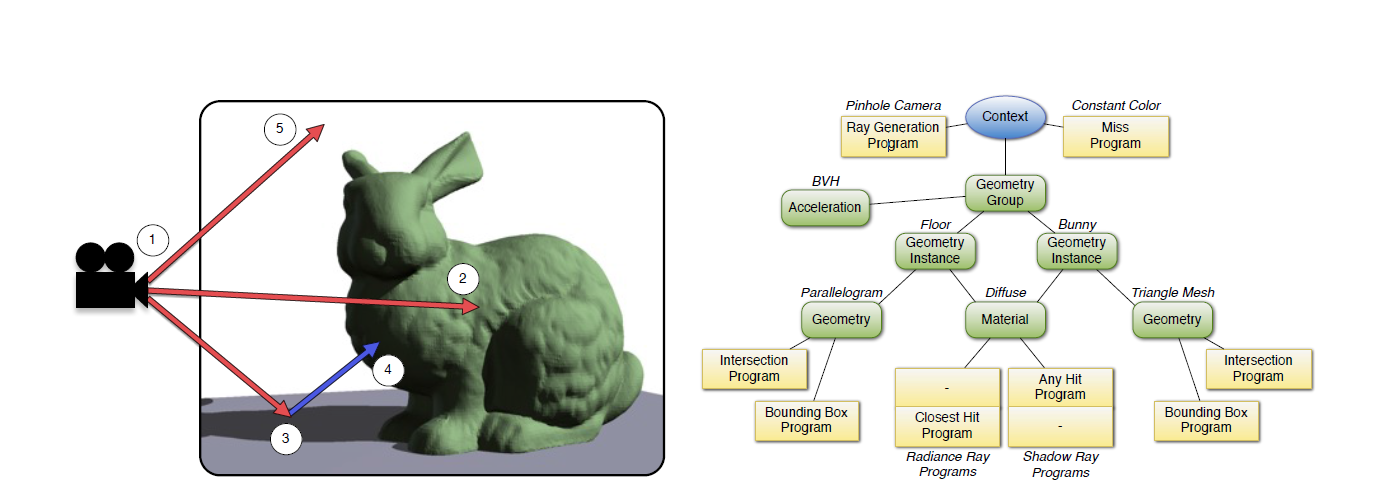
\includegraphics[width=1\linewidth]{fig1.png}}
\caption{Право: полный контекст OptiX для простой сцены с камерой с точечной диафрагмой, двумя объектами и тенями. Программа генерации луча реализует камеру, в то время как программа мисс реализует постоянный белый фон. Единственная группа геометрии содержит два экземпляра геометрии с единственным BVH, созданным по всей базовой геометрии в треугольной петле и плоскости основы. Два типа геометрии реализованы, треугольная петля и параллелограм, каждый с их собственным набором программ ограничивающего прямоугольника и перекрестка. Два экземпляра геометрии совместно используют единственный материал, который реализует рассеянную модель распространения света и полностью ослабляет теневые лучи через самый близкий хит и любой хит
программы, соответственно. Оставленный: Выполнение программ. 1. Программа генерации луча создает лучи и прослеживает их против группы геометрии, которая инициирует обход BVH. 2. Если луч пересечется с геометрией, то самую близкую программу хита вызовут после того, как очко жизни найдено.
3. Материал породит теневые лучи и проследит их против геометрии сцены. 4. Когда перекресток вдоль теневого луча будет найден, любая программа хита завершит обход луча и возвратится к программе вызова с теневой информацией. 5. Если луч не пересечется ни с какой геометрией сцены, то программу мисс вызовут.}
\label{fig1}
\end{figure}

Материальные объекты содержат информацию о штриховке операций, включая программы призывал к каждому перекрестку, поскольку они обнаружены (любая программа хита) и для перекрестка, самого близкого к источнику данного луча (самая близкая программа хита).

\subsubsection {Объектная модель и модель данных}
OptiX использует объектную модель специального назначения, разработанную, чтобы минимизировать постоянные данные, используемые программируемыми операциями. В отличие от системы OpenGL, где только единственная комбинация программ построения теней используется за один раз. Однако трассировка лучей может в произвольном порядке получить доступ к объектным и материальным данным. 

Поэтому, вместо универсальных переменных, используемых языками штриховки OpenGL, OptiX позволяет любому из объектов и узлов, описанных выше переносить произвольное набор переменных, выраженных как введенная пара значение-имя, вызывал переменную. Переменные установлены клиентским приложением и имеют доступ только для чтения во время выполнения трассировки. Переменные могут иметь скалярные или векторные целочисленные и типы с плавающей точкой (например, float3, int4), а также определяемый пользователем structs и ссылки на буферы и текстурировать сэмплеры. Механизм наследования для этих переменных уникален для OptiX. Вместо основанной на классе модели наследования с синглом сам или этот указатель, механизм OptiX отслеживает текущую геометрию и материальные объекты и текущий пересекающийся узел. Значения переменных наследованы от объектов, которые активны в каждой точке в потоке управления.

  Например, программа перекрестка наследует определения от геометрия и объекты экземпляра геометрии, в дополнение к глобальным переменным определены в контексте. Концептуально, OptiX исследует каждый из этих объектов для соответствующей пары имя/значение, когда к переменной получают доступ. Этот механизм может считаться обобщением вложенное определение объема найдено в большинстве языков программирования. Это может также быть реализовано вполне эффективно в своевременном компиляторе. Как пример того, как это полезно, полагайте, что массив источников света вызывал световые сигналы. Как правило, пользователь определил бы световые сигналы в контексте, глобальной области видимости OptiX. Это делает это значение доступным во всех программах построения теней во всей сцене. Однако, если световые сигналы для определенная объектная потребность, которая будет переопределена, другая переменная того же имени может быть создана и присоединена к экземпляру геометрии, связанному с тем объектом. Таким образом программы, соединенные с тем объектом, использовали бы переопределенное значение световых сигналов, а не значение, присоединенное к контексту. Это - мощный механизм, который может использоваться, чтобы минимизировать данные сцены, чтобы включить высокую производительность на архитектуре с минимальными кэшами. Способ, которым обработаны эти случаи, может измениться существенно от одного средства рендеринга до другого, таким образом, механизм OptiX обеспечивает основную функциональность, чтобы выразить любого число переопределения управляет эффективно.

Специальный тип переменной, тегированной с атрибутом ключевого слова, может использоваться, чтобы передать информацию от программы перекрестка до самого близкого - и любого - программы хита. Они походят на OpenGL переменные переменные и используются для передачи координат текстуры, normals и другой информации о штриховке от программ перекрестка до программ штриховки. У этих переменных есть специальная семантика — они записаны программой перекрестка, но только значения, связанные с самым близким перекрестком, сохранены. Этот механизм позволяет работе перекрестка быть абсолютно отдельной от операций штриховки, включая многократные одновременные примитивы и/или форматы хранения петли при тихой поддержке текстурирования, заштриховывая normals, и объектных искривлений для дифференциалов луча. Атрибуты, которые не используются никем самым близким - или любым - программа хита, могут игнорироваться компилятором OptiX.
\subsubsection {Динамическая отправка}
Чтобы позволить многократным операциям трассировки лучей сосуществовать в единственном выполнении, OptiX использует определяемый пользователем тип луча. Тип луча - просто индекс, который выбирает определенный набор слотов для любого хита и самых близких программ хита, которые будут выполняться, когда перекресток найден. Это может использоваться, например, чтобы рассматривать теневые лучи отдельно от другого
лучи. Точно так же многократные точки входа в контексте OptiX включают эффективному способу представлять различные передачи по тому же набору геометрии. Например, картопостроитель фотона может использовать одну точку входа, чтобы бросить фотоны в сцену и вторую точку входа, чтобы бросить лучи просмотра.
\subsubsection{Буферы и текстуры}
Ключевая абстракция для объемного хранения данных - многомерный буферный объект, который представляет 1-, 2-или 3-мерный массив фиксированного размера элемента. К буферу получают доступ через объект обертки C++ в любой из программ. Буферы могут быть только для чтения, только для записи или чтение-запись и поддерживать атомарные операции, когда поддерживается аппаратными средствами. Буфер основан на дескрипторе и не представляет необработанные указатели, таким образом позволяя времени выполнения OptiX переместить буферы для уплотнения хранения, или для продвижения другим пространствам памяти для производительности.
Буферы обычно используются для выходных изображений, треугольных данных,списки источника света и другие основанные на массиве данные. Буферы - единственные средства данных вывода из программы OptiX. В большинстве приложений программа генерации луча будет ответственна за запись данных к буферу вывода, но любой из программ OptiX позволяют записать в буферы вывода в любом расположении, но без упорядочивания гарантий.

Буфер может также быть связан с объектом сэмплера текстуры, который использует GPU, текстурирующий аппаратные средства. Буферы и объекты сэмплера текстуры связаны с переменными OptiX и используют те же механизмы определения объема как значения программы построения теней. Кроме того, оба буфера и сэмплеры текстуры могут взаимодействовать с OpenGL и DirectX, включая эффективную реализацию гибридных приложений растеризации/трассировки лучей.
\subsection{системных обзора}
Механизм OptiX состоит из двух отличных ПЧЕЛ, один для стороны узла и один для кода 1 стороны устройства, API узла - ряд C функции, что вызовы клиентского приложения, чтобы создать и сконфигурировать контекст, соберите график узла и запустите ядра трассировки лучей. Это также обеспечивает вызовы, чтобы управлять устройствами, используемыми для выполнения ядра. API программы - функциональность, представленная пользовательским программам. Это включает вызовы функции для трассировки лучей, сообщая о перекрестках, и доступ к данным. Кроме того, несколько семантических переменных кодируют состояние, определенное для трассировки лучей, например, текущее расстояние до самого близкого перекрестка.
Печать и средства обработки исключений также доступна для отладки.

Рисунок 5 обрисовывает в общих чертах поток управления приложения OptiX. Во время установки приложение вызывает API-функции узла OptiX, чтобы обеспечить данные данных сцены, такие как геометрия, материалы, ускоряющие структуры, иерархические отношения и программы. Последующий вызов к rtContextLaunch API-функции передает управление к OptiX, где изменения в контексте обработаны. При необходимости новое ядро трассировки лучей скомпилировано из данных пользовательских программ. Ускоряющие структуры созданы (или обновлены), и данные синхронизируются между памятью устройства и узлом. Наконец, ядро трассировки лучей выполняется, вызывая различные пользовательские программы, как описано в Разделе 3. После того, как выполнение ядра трассировки лучей закончилось, его данные результата могут использоваться приложением. Как правило, это включает чтение от буферов вывода, заполненных одной из пользовательских программ или отображения такого буфера непосредственно, например, через OpenGL. Интерактивное или многопроходное приложение тогда повторяет процесс, запускающийся при установке контекста, где произвольные изменения в контексте могут быть внесены, и ядро запущено снова.
\subsection{ускоряющих структур}
Базовый алгоритм для нахождения перекрестка между лучом и геометрией сцены включает обход ускоряющих структур. Такие структуры данных - жизненный компонент фактически каждой системы трассировки лучей. Они - обычно пространственные или иерархии объектов и используются пересекающимся алгоритмом, чтобы эффективно искать примитивы
это потенциально пересекает данный луч. OptiX предлагает гибкий интерфейс, подходящий для широкого диапазона приложений, чтобы управлять его ускоряющими структурами.
\subsubsection{Взаимодействие с графиком узла}
Одна из причин сбора данных геометрии в графике узла состоит в том, чтобы упростить организацию связанных ускоряющих структур. Вместо того, чтобы поддержать всю геометрию сцены в единственной ускоряющей структуре, это часто целесообразно создавать несколько структур по различным областям сцены. Например, части сцены могут быть анимированы, требуя, чтобы ускоряющая структура была восстановлена для каждой передачи трассировки лучей. В этом случае создание отдельной структуры для статических областей сцены может увеличить эффективность. В дополнение к только построению статической структуры один раз, приложение может обычно инвестировать больший бюджет времени в более высокую качественную сборку.

\begin{figure}[h!]
\center{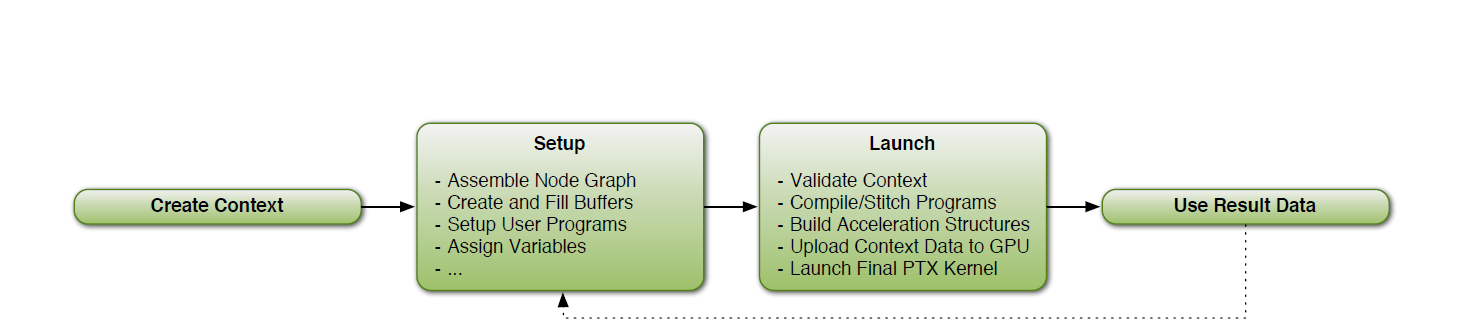
\includegraphics[width=1.1\linewidth]{fig2.png}}
\caption{Основной поток управления приложения OptiX. Отдельными шагами во время установки контекста управляет приложение, процедура запуска обработана OptiX.}
\label{fig2}
\end{figure}
  Механизм OptiX связывает ускоряющие структуры со всеми группами и группы геометрии в графике узла. Структуры, присоединенные к группам геометрии, являются низким уровнем, созданным по геометрическим примитивам, которые содержит группа геометрии. Структуры на группах созданы по границам дочерних элементов той группы и таким образом представляют ускоряющие структуры высокого уровня. Эти структуры высокого уровня полезны, чтобы выразить иерархические отношения между геометрией, которая изменена на различных уровнях. 
  
 \paragraph{Инстанцирование.} Важной целью проекта для ускоряющей системы структуры была поддержка гибкого инстанцирования. Здесь, инстанцирование относится к репликации низких издержек геометрии сцены, ссылаясь на те же данные несколько раз, не имея необходимость копировать тяжелые структуры данных. Как описано в Разделе 3.2.1, на узлы в графике можно сослаться многократно, который естественно реализует инстанцирование. Это желательно к не, только делятся информацией геометрии среди экземпляров, но и ускоряющими структурами также. Одновременно, должно быть возможно присвоить данные негеометрии, такие как материальные программы и переменные независимо для каждого экземпляра. 
  
  Мы принимали решение представить ускоряющие структуры, поскольку отдельный API возражает, что присоединены к группам и группам геометрии. В случае инстанцирования возможно присоединить единственную ускоряющую структуру к многократным узлам, таким образом совместно используя ее данные и избегая избыточной конструкции той же структуры данных. Метод также приводит к эффективному дополнению и удалению экземпляров во времени выполнения. Рисунок 6 показывает пример графика узла с инстанцированием.
\paragraph{Ускоряющие структуры на объединенной геометрии.} Деление сцены в многократные ускоряющие структуры уменьшает время сборки структуры, но также и уменьшает производительность обхода луча. В ограничивающем случае полностью статической сцены можно было бы обычно выбирать сингл ускоряющая структура. Одна идея позади ускоряющих структур на группах геометрии состоит в том, чтобы упростить управление данными приложения для того типа установки: вместо того, чтобы иметь необходимость объединить геометрического человека объекты в монолитный блок, они могут остаться организованными как отдельные конфигурации и экземпляры, и легко быть собраны в единственной группе геометрии. Соответствующая ускоряющая структура будет создана по отдельным примитивам любых геометрических объектов, приводящих к максимальной производительности, как будто вся геометрия была объединена.

\begin{figure}[h!]
\center{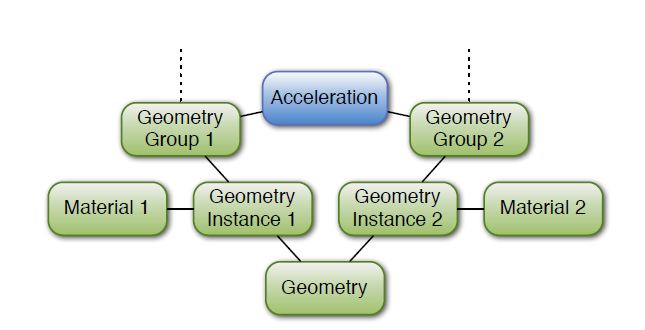
\includegraphics[width=0.5\linewidth]{fig3.png}}
\caption{График узла с инстанцированием. И группы геометрии ссылаются на тот же объект геометрии и совместно используют ускоряющую структуру, но используют различные материалы. Данные геометрии не дублированы..}
\label{fig3}
\end{figure}
Механизм OptiX будет внутренне заботиться о необходимых бухгалтерских задачах, таких как корректное переотображение существенных индексов.

  Группа геометрии может также использовать определенную информацию за объект при создании ее ускоряющей структуры. Например, в группе геометрии, содержащей многократные объекты, только единственный, возможно, был изменен между передачами трассировки лучей. OptiX может принять во внимание та информация и опускает некоторые избыточные операции (например.вычисления ограничивающего прямоугольника, посмотрите Раздел 5.3).
\subsubsection{Типы ускоряющих ускоряющих структур}
 Трассировки лучей структур - активная область исследования.Нет никакого единственного типа, который оптимален для всех приложений при всех условиях. Типичный компромисс между различными вариантами - производительность трассировки лучей по сравнению со скоростью конструкции, и у каждого приложения есть различный оптимальный баланс. Поэтому, OptiX обеспечивает много различных ускоряющих типов структуры что приложение может выбрать из. Каждая ускоряющая структура в графике узла может иметь другой тип, позволяя комбинации высококачественных статических структур с динамично обновленными. Большинство типов также подходит для структур высокого уровня, т.е. ускоряющих структур, присоединенных к группам.

В настоящее время реализованные ускоряющие структуры включают алгоритмы, фокусируемые на качестве иерархии (например, SBVH [Штих и др. 2009]) на скорости конструкции (например, LBVH [Лаутербах и др. 2009]), и различные промежуточные уровни баланса.
\subsubsection{Конструкция}
Каждый раз, когда базовая геометрия ускоряющей структуры изменена, например, во время анимации, она явно отмечена для, восстанавливают клиентским приложением. OptiX тогда создает так запланированные ускоряющие структуры на последующем вызове rtContextLaunch API-функции. 

Первая стадия в ускоряющей конструкции структуры получает ограничивающие прямоугольники геометрии, на которую ссылаются. Это достигнуто, выполняя для каждого геометрического примитива в объекте программу ограничивающего прямоугольника, описанную в Разделе 3.1, который требуется, чтобы возвращать консерватора выровненный осью ограничивающий прямоугольник для его примитивного ввода.Используя эти ограничивающие прямоугольники как элементарные примитивы для ускоряющих структур обеспечивает необходимую абстракцию, чтобы проследить лучи против произвольной определяемой пользователем геометрии (включая несколько типов геометрии в единственной структуре). Чтобы получить необходимые ограничивающие прямоугольники для высокоуровневых узлов группы в дереве, объединение примитивных ограничивающих прямоугольников сформировано и распространено рекурсивно.

Второй этап конструкции состоит из фактического создания требуемых ускоряющих структур, данных полученные ограничивающие прямоугольники.Доступный узел и параллелизм устройства могут быть использованы двумя способами. Во-первых, многократные ускоряющие структуры в графике узла могут быть созданы параллельно, поскольку они независимы. Во-вторых, единственный ускоряющий код сборки структуры может обычно параллелизироваться (см., например, [Шевцов и др. 2007], [Чжоу и др. 2008], [Лаутербах и al.2009]). Заключительные ускоряющие данные структуры помещены в память устройства для потребления кодом обхода луча.
\subsubsection{Настройка}
В то время как ускоряющие структуры в механизме OptiX разработаны, чтобы выполнить хорошо из поля, иногда необходимо для приложения предоставить дополнительную информацию, чтобы достигнуть максимально возможной производительности. Приложение может поэтому установить ускорение специфичные для структуры свойства, которые влияют на последующие сборки структуры и излучают обходы.

  Один пример для такого свойства - флаг “ремонта”: если геометрия, используемая ускоряющей структурой BVH, изменилась только немного, часто достаточно просто переоборудовать внутренние ограничивающие прямоугольники BVH вместо того, чтобы восстановить полную структуру с нуля (см. [Лаутербах и др. 2006]). Клиентское приложение может включить это поведение на определенных типах ускоряющих структур, если это предполагает, что получающееся общее время выполнения уменьшится. Такие решения оставляют приложению, поскольку оно обычно обладает контекстной информацией, которая недоступна к OptiX.
  
    Процедуры сборки, специализированные к определенным типам геометрических примитивов (в противоположность выровненным осью ограничивающим прямоугольникам, обсужденным выше), являются вторым случаем, где свойства полезны. Приложение может, например, сообщить, что ускорение SBVH structureиthat базовая геометрия состоит исключительно из треугольников, и где эти треугольники расположены в памяти. SBVH может тогда выполнить более точный метод построения иерархии, которая приводит к более высокому качеству.
    
\subsection{проблемно-ориентированных компиляций}
Ядро времени выполнения узла OptiX - Своевременный (JIT) компилятор, который обеспечивает несколько важных частей функциональности. Во-первых, этап JIT комбинирует все предоставленные пользователями программы программы построения теней в одно или более ядер. Во-вторых, это анализирует график узла, чтобы идентифицировать информационно-зависимую оптимизацию. В-третьих, это обеспечивает зависящий от домена Двоичный интерфейс приложений (ABI) и модель выполнения, которая реализует рекурсию и операции указателя функции на устройстве, которое естественно не поддерживает их. Наконец, получающееся ядро выполняется на GPU, используя API драйвера CUDA.
\subsubsection{Программы OptiX}
Определенные пользователями программы, часто называемые программой построения теней, обеспечены для API узла OptiX в форме Параллельного Выполнения Потока (PTX) функции [NVIDIA 2010b]. PTX - ассемблер виртуальной машины, который является частью архитектуры CUDA. Это реализует низкоуровневую виртуальную машину, подобную во многих отношениях популярному промежуточному представлению Low-Level Virtual Machine (LLVM) с открытым исходным кодом [Lattner и Adve 2004]. Как LLVM, PTX определяет ряд простых инструкций, которые обеспечивают основные операции для арифметики, потока управления и доступа к памяти. 

PTX также обеспечивает несколько высокоуровневых операций, таких как доступ текстуры и трансцендентальные операции. Также подобный LLVM, PTX принимает бесконечный регистровый файл и краткие обзоры много реальных машинных команд. JIT-компилятор во времени выполнения CUDA выполнит выделение регистра, планирование инструкции, устранение невыполняемого кода и многочисленную другую последнюю оптимизацию, поскольку это производит машинный код, предназначающийся для определенной архитектуры GPU.
PTX записан с точки зрения единственного потока и таким образом не требует явных операций манипулирования маской маршрута. Это делает его прямым, чтобы понизить PTX с высокоуровневого языка штриховки при предоставлении времени выполнения OptiX возможности управлять и оптимизировать получающийся код.

  В то время как это обеспечивает мощный основанный на С++ язык штриховки, это может не быть полезно во всех приложениях. Альтернативно, любой фронтэнд компилятора, который может испустить PTX, мог использоваться. Можно было вообразить фронтэнды для Cg, HLSL, GLSL, MetaSL, OpenSL, RSL, GSL, OpenCL, и т.д., который мог произвести надлежащий PTX для ввода в OptiX. Этим способом OptiX - агностик языка штриховки, так как многократные варианты синтаксиса могли использоваться, чтобы генерировать программы для использования с API во время выполнения.
\subsubsection{PTX к компиляции PTX}
Учитывая набор функций PTX для определенной сцены, компилятор OptiX переписывает PTX использование многократного PTX к передачам преобразования PTX, которые подобны передачам компилятора, которые оказались успешными в инфраструктуре LLVM. Этим способом OptiX использует PTX в качестве промежуточного представления, а не традиционной системы команд. Этот процесс реализует много проблемно-ориентированные операции включая ABI (вызывающая последовательность), разовая ссылкой оптимизация и информационно-зависимая оптимизация. Факт, что большинство структур данных в типичном трассировщике лучей только для чтения, обеспечивает существенную возможность для оптимизации, которую не считали бы безопасной в более общей среде.
\paragraph{ Анализ.} 
Первая стадия этого процесса должна выполнить статический анализ всех обеспеченных функций PTX. Эта передача гарантирует, что переменные, на которые ссылаются в каждой функции, были обеспечены
графиком узла и имеют непротиворечивые типы. Одновременно, мы определяем, только для чтения ли каждый из буферов данных или чтение-запись, чтобы сообщить времени выполнения, где данные должны храниться. Наконец, эта передача может проанализировать структуру графика узла в подготовке к другой специфичной для данных оптимизации, показанной ниже.
\paragraph{ Встройте instrinsic операции.} 
Время выполнения OptiX обеспечивает несколько операций вне тех предоставленных CUDA. Эти инструкции заменены встроенной функцией, которая реализует требуемые операции. Примеры включают доступ к в настоящее время активному источнику луча, направлению и полезной нагрузке, абстракции хранилища поверхности записи чтения и доступу к стеку преобразования. Кроме того, мы обрабатываем псевдо инструкции, соответствующие исключительному потоку управления, такие как rtTerminateRay и rtIgnoreIntersection. 
\paragraph{Объектная модель переменной программы построения теней.}
 Программа может сослаться на a переменная программы построения теней без дополнительного синтаксиса, так же, как к задействованной переменной получили бы доступ в C++. Эти доступы проявят в PTX как инструкция загрузки, связанная со специально теговыми глобальными переменными.
Мы обнаруживаем доступы к этим переменным, используя анализ потока данных, передают и заменяют их загрузкой, индексированной от указателя до текущей геометрии, материала, экземпляра или другого объекта API, как определено аналитической передачей. Чтобы реализовать динамическое наследование переменных, маленькая таблица, связанная с каждым объектом, определяет указатель базы и связанное смещение.

\begin{verbatim}
for( int i = 0; i < 5; ++i ) {
Ray ray = make_Ray( make_float3( i, 0, 0 ),
make_float3( 0, 0, 1 ),
0, 1e-4f, 1e20f );
UserPayloadStruct payload;
rtTrace( top_object, ray, payload );
}
\end{verbatim}
ПОДПИСЬA simple CUDA C program snippet that calls rtTrace, a function that requires a continuation, in a loop.
\begin{verbatim}
ld.global.u32\%node, [top_object+0];
mov.s32 \%i, 0;
loop:
call _rt_trace, ( \%node,\%i, 0, 0, 0, 0, 1,
0, 1e-4f, 1e20f, payload );
add.s32 \%i, \%i, 1;
mov.u32 \%iend, 5;
setp.ne.s32 \%predicate, \%i, \%iend;
@\%predicate bra loop;
\end{verbatim}
ПОДПИСЬКод PTX, соответствующий программе в рисунке 7. Регистр \%i жив через вызов к rtTrace. Поэтому, механизм продолжения должен восстановить его после возвратов вызова.

\paragraph{Продолжения.} Считайте программу программы построения теней показанной в рисунке 7 и соответствующем PTX показанный в рисунке 8. Эта программа реализует простой цикл, чтобы проследить 5 лучей от точек (0,0,0), (1,0,0), (2,0,0), (3,0,0) и (4,0,0). В то время как не полезная программа, этот пример может использоваться, чтобы проиллюстрировать, как используются продолжения. Чтобы позволить этому циклу выполняться как ожидалось, переменная, я должен быть спасен прежде временно отказываясь от выполнения этой программы, чтобы вызвать функцию rtTrace. 

Это выполнено, реализовывая отсталую аналитическую передачу потока данных, чтобы определить регистры PTX, которые живы, когда с псевдоинструкцией для rtTrace встречаются. Живой регистр - тот, который используется в качестве параметра за некоторую последующую инструкцию в графе потоков данных. Мы резервируем слоты на стеке для каждой из этих переменных, упаковываем их в 16-байтовые векторы, если это возможно, и храним их на стеке перед вызовом и восстанавливаем их после вызова. Это подобно ABI сохранения вызывающая сторона, который традиционный компилятор реализовал бы для основанного на ЦП языка программирования. В подготовке к представлению продолжений мы выполняем поднимающую цикл передачу, и распространение копии передают каждую функцию, чтобы помочь минимизировать состояние, сохраненное в каждом продолжении. 

Наконец, rtTrace псевдоинструкция заменена ответвлением, чтобы возвратить выполнение конечному автомату, описанному ниже, и метка, которая может использоваться, чтобы в конечном счете возвратить поток управления этой функции. Это преобразование приводит к псевдокоду, показанному в рисунке 9.
Однако неструктурный gotos в этом коде приведет к неприводимому графику потока управления из-за ввода цикла и наверху цикла и наверху метки state2.

Неприводимый поток управления мешает механизмам в GPU, чтобы управлять выполнением SIMD этой функции, приводящей к драматическому замедлению для расходящегося кода. Следовательно, мы разделяем эту функцию, клонируя узлы в графике для каждого состояния. После выполнения устранения невыполняемого кода получена кодовая последовательность в рисунке 10.Этот поток управления более дружественный по отношению к выполнению SIMD, потому что это хорошо структурировано. Расхождение может быть далее уменьшено, представляя новые состояния вокруг общего кода. Это заключительное преобразование может или может не стоить, в зависимости от стоимости переключения состояний и степени расхождения выполнения.
\begin{verbatim}
state1:
for( int i = 0; i < 5; ++i ) {
Ray ray = make_Ray( ..., i, ... );
UserPayloadStruct payload;
push i;
state = trace;
goto mainloop;
state2:
pop i;
}
\end{verbatim}
ПОДПИСЬPseudo-code for the program in Figure 7 with inserted continuation.
\begin{verbatim}
state1:
i = 0;
Ray ray = make_Ray( ..., i, ... );
UserPayloadStruct payload;
push i;
state = trace;
goto mainloop;
state2:
pop i;
++i;
if( i > 5 ) {
state = returnState;
goto mainloop;
}
Ray ray = make_Ray( ..., i, ... );
UserPayloadStruct payload;
state = trace;
goto mainloop;
\end{verbatim}
ПОДПИСЬПсевдокод для программы в рисунке 7 с продолжением и разделением, чтобы возвратить приводимость графика потока управления.

\subsubsection{Оптимизация}
Инфраструктура компилятора OptiX обеспечивает ряд проблемно-ориентированной и информационно-зависимой оптимизации, которая была бы сложна, чтобы реализовать статически скомпилированную среду. Они включают (увеличения производительности для множества приложений в круглых скобках):

• Игнорируйте операции преобразования для графиков узла, которые не используют узел преобразования (до 7\%-го повышения производительности).

• Устраните печать и исключение связанный код, если эти опции не включены в текущем выполнении.

• Уменьшите размер продолжения, регенерируя константы и промежуточные звенья после восстановления. Так как модель выполнения OptiX гарантирует, что объектно-специфичные переменные только для чтения, эта локальная оптимизация не требует межпроцедурной передачи.

• Специализируйте обход на основе древовидных характеристик, таких как существование вырожденных листов, вырожденных деревьев, совместно используемых ускоряющих данных структуры, или смешал типы примитивов.

• Переместите маленькие данные только для чтения в постоянную память или текстуры, если есть свободное место (до 29\%-го повышения производительности).

Кроме того, передачи перезаписи могут представить существенные модификации коду, который может быть очищен дополнительными стандартными оптимизационными проходами, такими как устранение невыполняемого кода, постоянное распространение, подъем цикла и распространение копии.
\begin{verbatim}
state = initialState;
while( state != DONE )
switch(state) {
case 1: state = program1(); break;
case 2: state = program2(); break;
...
case N: state = programN(); break;
}
\end{verbatim}
ПОДПИСЬПсевдокод для простого конечного автомата приближается к выполнению мегаядра. Состояние, которое будет выбрано затем, выбрано оператором переключения. Переключатель неоднократно выполняется, пока переменная состояния не содержит специальное значение, которое указывает завершение.

\subsection{ моделей выполнения}
Различные авторы предложили различные модели выполнения для параллельной трассировки лучей. В частности монолитное ядро или мегаядро, подход оказывается успешным на современном GPUs [Эйла и Лэн 2009]. Этот подход минимизирует запуск ядра наверху, но потенциально уменьшает использование процессора, когда требования регистра растут к максимуму через составляющие ядра. Поскольку задержка при обращении к памяти маски GPUs с многопоточностью, это - тонкий компромисс.
OptiX реализует мегаядро, соединяя ряд отдельных пользовательских программ и пересекая конечный автомат, вызванный потоком выполнения между ними во времени выполнения.

  Поскольку GPUs развиваются, различные модели выполнения могут стать практичными. Например, модель выполнения потоковой передачи [Gribble и Ramani 2008] может быть полезной на некоторой архитектуре. Другая архитектура может обеспечить поддержку аппаратных средств для ускоряющего обхода структуры или других общих операций. Так как механизм OptiX не предписывает, чтобы порядок выполнения между корнями деревьев луча, эти альтернативы могли быть предназначены с передачей перезаписи, подобной той, мы в настоящее время используем, чтобы генерировать мегаядро.
\subsubsection{ Выполнение мегаядра}
Прямой подход к выполнению мегаядра - простая итерация по конструкции случая переключателя. В каждом случае выполняется пользовательская программа, и результат этого вычисления имеет место, или состояние, чтобы выбрать на следующей итерации. В таком механизме конечного автомата OptiX может реализовать вызовы функции, рекурсию и исключения.
Рисунок 11 иллюстрирует простой конечный автомат. Состояния программы просто вставлены в тело оператора переключения. Государственный индекс, который мы вызываем виртуальный счетчик команд (VPC), выбирает отрывок программы, который будет выполняться затем. Вызовы функции реализованы устанавливая VPC непосредственно, вызовы виртуальной функции реализованный, устанавливая его от таблицы и функциональных возвратов просто восстанавливают состояние к продолжению, связанному с ранее активной функцией (виртуальный обратный адрес). Кроме того, специальный поток управления, такой как исключения управляет VPC непосредственно, создавая переход требуемого состояния способом, подобным легкой версии setjmp / longjmp функциональность, обеспеченная C.
\subsubsection{ Мелкомодульное планирование}
В то время как прямой подход к выполнению мегаядра функционально корректен, это переносит штрафы сериализации, когда состояние отличает в единственном модуле SIMT [Линдхольма и др. 2008]. Чтобы смягчить эффекты расхождения выполнения, время выполнения OptiX использует мелкомодульную схему планирования исправить расходящиеся потоки
это было бы, иначе бездействовал. Вместо того, чтобы позволить аппаратным средствам SIMT автоматически сериализировать выполнение расходящегося переключателя, 
\begin{verbatim}
state = initialState;
while( state != DONE ) {
next_state = scheduler();
if(state == next_state)
switch(state) {
// Insert cases here as before
}
}
\end{verbatim}
ПОДПИСЬПсевдокод для выполнения мегаядра через конечный автомат с мелкомодульным планированием.
\begin{figure}[h!]
\center{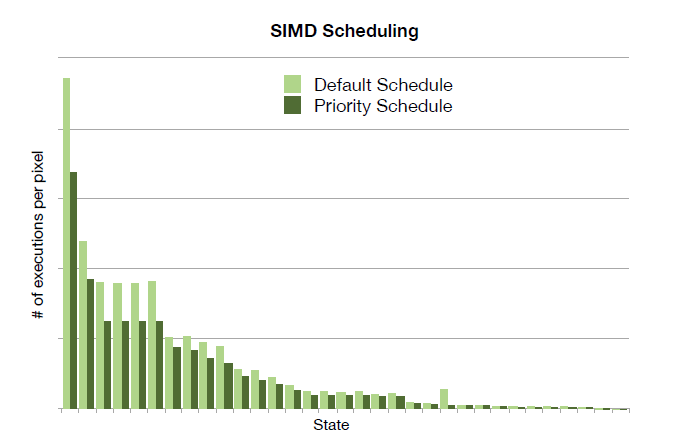
\includegraphics[width=0.8\linewidth]{fig4.png}}
\caption{Преимущество мелкомодульного планирования с установлением приоритетов.Панели представляют число государственного выполнения за пиксель. Существенное сокращение может быть замечено, планируя изменения состояния с фиксированным приоритетом, как описано в Разделе 7.2.}
\label{fig4}
\end{figure}
OptiX явно выбирает единственное состояние для всего модуля SIMT, чтобы выполнить использование эвристики планирования. Потоки в модуле SIMT, которые не требуют состояния просто, бездействуют та итерация. Механизм обрисован в общих чертах в рисунке 12.

Мы экспериментировали со множеством мелкомодульной эвристики планирования. Одна простая схема, которая работает хорошо, определяет расписание, присваивая статическое установление приоритетов по состояниям. Планируя потоки с подобными состояниями во время выполнения, OptiX сокращает количество общих изменений состояния, сделанных модулем SIMT, который может существенно
уменьшите время выполнения по автоматическому расписанию, вызванному аппаратными средствами сериализации. Рисунок 13 показывает пример такого сокращения.
\subsubsection{ Выравнивание нагрузки}
В дополнение к уменьшению расхождения выполнения SIMT с мелкомодульным планировщиком OptiX использует трехярусный подход балансирования динамической нагрузки к GPUs. Каждый запуск ядра трассировки лучей представлен как очередь задач параллели данных к физическим модулям выполнения. Текущая модель выполнения осуществляет независимость между
эти задачи, позволяя балансировщику загрузки динамично запланировать работу на основе характеристик рабочей нагрузки и аппаратных средств выполнения.

Работа распределена от узла ЦП до одного или более GPUs динамично, чтобы включить крупномодульное выравнивание нагрузки между GPUs отличающейся производительности. Как только пакет работы был представлен GPU, это помещено в глобальную очередь. Каждый модуль выполнения на GPU присвоен локальная очередь, которая переполнена от глобальной очереди GPU и динамично распределяет работу отдельным элементам обработки, когда они завершили свое текущее задание. 
\begin{figure}[h!]
\center{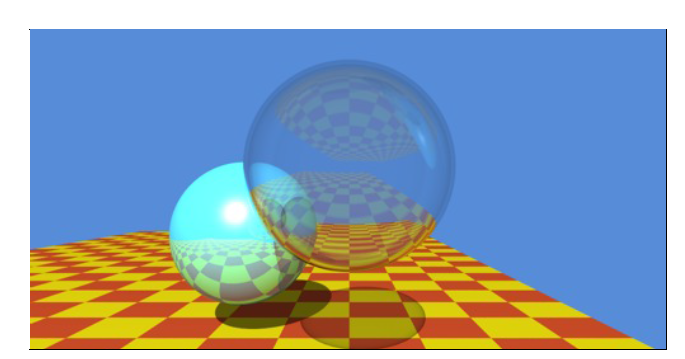
\includegraphics[width=0.8\linewidth]{fig5.png}}
\caption{Воссоздание сцены сферы Виттеда с userspecified программы: сфера и прямоугольный перекресток; стеклянное, процедурное средство проверки и металлические программы хита; небо программа мисс; и камера с точечной диафрагмой с адаптивным сглаживанием излучает генерацию. Выполнения в более чем 30 кадр/с на GeForce GTX480 в 1k 1k разрешением.}
\label{fig5}
\end{figure}
Это - расширение схемы, используемой [Эйла и Лэн 2009], чтобы включить динамическую нагрузку, балансирующуюся между GPUs.

\subsection{тематических исследований приложения}
Этот раздел представляет различные варианты использования OptiX, обсуждая основные идеи позади многих различных приложений.

\subsubsection{Whitted-разработайте трассировку лучей}
OptiX SDK содержит несколько приложений трассировки лучей в качестве примера. Один из них - обновленное воссоздание исходной сцены сферы Виттеда [1980]. Эта сцена проста, все же демонстрирует важные функции механизма OptiX.

Программа генерации луча выборки реализует основную модель камеры с точечной диафрагмой. Позиция камеры, ориентация и видимое пространство определены рядом переменных программы, которые могут быть изменены в интерактивном режиме. Программа генерации луча начинает процесс штриховки, стреляя в единственный луч за пиксель или, по пользовательскому запросу, выполняя адаптивное сглаживание через избыточную выборку. Материальные самые близкие программы хита тогда ответственны за то, что рекурсивно бросили лучи и вычислили теневой демонстрационный цвет. После возврата из рекурсии программа генерации луча накапливает демонстрационный цвет, сохраненный в полезной нагрузке луча, в буфер вывода.

Приложение определяет трех отдельных пар перекрестка и программ ограничивающего прямоугольника, каждый реализующий различный геометрический примитив: параллелограм для пола, сфера для металлического шара и сфера тонкой оболочки для полого стеклянного шара. Стеклянный шар, возможно, был смоделирован с двумя экземплярами простой примитивной сферы, но гибкость модели программы OptiX дает нам свободу реализовать более эффективную специализированную версию для этого случая. Каждая программа перекрестка устанавливает несколько переменных атрибута: геометрическое нормальное, нормальная штриховка, и, при необходимости координата текстуры. Атрибуты используются материальными программами, чтобы выполнить вычисления штриховки.

  Механизм типа луча используется, чтобы дифференцировать сияние от теневых лучей. Приложение присоединяет тривиальную программу, которая сразу завершает луч к любым слотам хита материалов для теневых лучей. Это раннее завершение луча приводит к высокой эффективности для взаимных тестов видимости между точкой штриховки и источником света.
стеклянный материал - исключение, однако: здесь, любая программа хита используется, чтобы ослабить фактор видимости, сохраненный в полезной нагрузке луча. В результате стеклянная сфера бросает более тонкую тень, чем металлическая сфера.
\begin{figure}[h!]
\begin{verbatim}
float3 throughput = make_float3( 1, 1, 1 );
payload.nextRay = camera.getPrimaryRay();
payload.shootNextRay = true;
while( payload.shootNextRay == true ) {
rtTrace( payload.nextRay, payload );
throughput *= payload.throughput;
}
sampleContribution = payload.lightColor * throughput;
\end{verbatim}
\caption{Псевдокод для итеративной трассировки пути в Гараже Проекта.}
\label{fig6}
\end{figure}
ПОДПИСЬ
\subsubsection{ Гараж проекта NVIDIA}
Гараж Проекта NVIDIA - сложная интерактивная демонстрация рендеринга, предназначенная для общедоступного распределения. Главное изображение рисунка 1 было представлено, используя это программное обеспечение. Ядро Гаража Проекта - физическая система трассировки пути Монте-Карло [Kajiya 1986], что постоянно демонстрационные световые пути и совершенствовали изображение оценка, интегрируя новые выборки в течение долгого времени. Пользователь может в интерактивном режиме просмотреть и отредактировать сцену, поскольку начальное шумное изображение сходится к окончательному решению.

Чтобы управлять использованием стека, Гараж Проекта реализует трассировку пути, используя итерацию в программе генерации луча вместо того, чтобы рекурсивно вызвать rtTrace. Псевдокод рисунка 15 подводит итог.
В Гараже Проекта каждый материал использует самую близкую программу хита, чтобы определить следующий луч, который будет прослежен и пасует назад это использование определенного поля в полезной нагрузке луча. Самая близкая программа хита также вычисляет пропускную способность текущего легкого возврата, который используется генерация луча, чтобы поддержать кумулятивный продукт пропускной способности по полному световому пути. Умножение цвета источника света, пораженного последним лучом по пути, приводит к заключительному демонстрационному вкладу.

Поддержка OptiX C++ в программах луча позволяет материалам совместно использовать универсальную самую близкую реализацию хита, параметризованную на тип BSDF. Это позволяет нам реализовывать новые материалы как классы BSDF с методами для выборки важности, а также BSDF и вероятности оценка плотности. Гараж проекта реализует число из различных физических материалов, включая металлическую и автомобильную краску. Некоторые из этих программ построения теней поддерживают нормальные и зеркальные карты.

В то время как OptiX реализует всю функциональность трассировки лучей Гаража Проекта, конвейер OpenGL реализует заключительную реконструкцию изображения и дисплей. Этот конвейер выполняет различные этапы обработки сообщения, такие как тональное отображение, блик и фильтрация стандарта использования основанные на растеризации методы.

\subsubsection{Отображение фотона пространства изображения}
Image Space Photon Mapping (ISPM) [Макгуайр и Луебк, 2009] является алгоритмом рендеринга в реальном времени, который комбинирует стратегии трассировки лучей и растеризации (рисунок 16). Мы портировали опубликованную реализацию на механизм OptiX. Тот процесс дает понимание различий между традиционным векторизованным последовательным трассировщиком лучей и OptiX.
\begin{figure}[h!]
\center{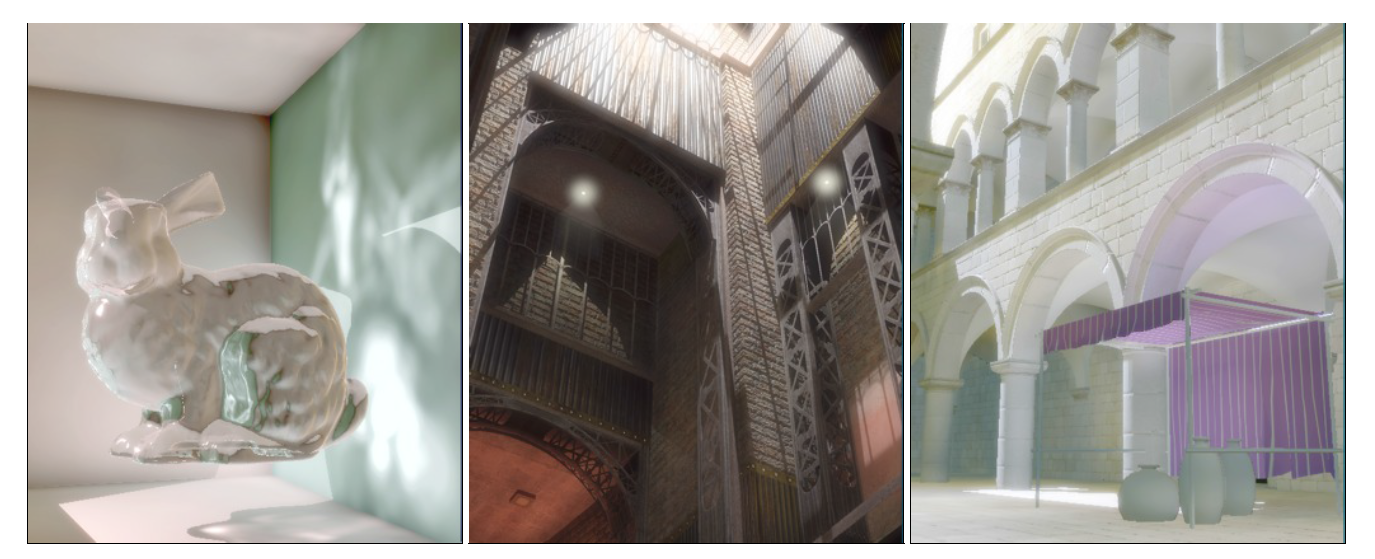
\includegraphics[width=1\linewidth]{fig6.png}}
\caption{ISPM глобальное освещение в реальном времени. Рекурсивная самая близкая программа хита в OptiX реализует трассировку фотона.}
\label{fig6}
\end{figure}
Алгоритм ISPM вычисляет первый сегмент путей фотона от света, растеризируя “карту возврата” от ссылочного фрейма света. Это тогда распространяет фотоны трассировкой лучей с Русской рулеткой, выбирающей до последнего события рассеивания перед глазом. В каждом событии рассеивания фотон депонирован в массив, который является “картой фотона”. Косвенное освещение тогда собрано в изображении пространство, растеризируя небольшой объем вокруг каждого фотона с точки зрения глаза. Прямое освещение вычислено схемами затенения и растеризацией.

Рассмотрите структуру трассировщика фотона ЦП-ISPM. Это запускает один персистентный поток за ядро. Эти потоки обрабатывают пути фотона от глобальной переменной, незапертого рабочего списка. Отображение фотона ISPM генерирует несвязные лучи, таким образом, традиционные пакетные стратегии векторизации обхода луча не помогают с этим процессом. Для каждого пути поток обработки вводит цикл с условием продолжения, внося один фотон в глобальной переменной, незапертом массиве фотона за итерацию. Цикл завершается после поглощения фотонов.

Под OptiX-ISPM мы также поддерживаем глобальные незапертые буферы ввода и вывода. Увеличения производительности трассировки с успехом мелкомодульного планирования программ в когерентные модули SIMT и уменьшения с размером состояния связывались между программами.Имитация традиционного стиля ЦП архитектуры программного обеспечения была бы неэффективна под OptiX, потому что это потребует передачи всех материальных параметров между генерацией луча и поразит программы и переменный итеративный цикл с условием продолжения в самой близкой программе хита. OptiXISPM поэтому следует альтернативному проекту, который рассматривает все распространение итерации как сопрограммы. Это содержит единственную программу генерации луча с одним потоком за путь фотона. Рекурсивная самая близкая программа хита реализует итерации распространять-и-вносить. Это позволяет потокам уступать между итерациями так, чтобы мелкомодульный планировщик мог перегруппировать их. 

Мы отмечаем, что широкий подход, проявленный здесь, является способом объединить API растровой графики как OpenGL или DirectX с примитивами трассировки лучей, не расширяя растровый API. Задержанная штриховка - форма получения, где буферы геометрии походят на functionalprogramming продолжение, которое содержит состояние прерванного пиксельный шейдер. Те буферы рассматривает как ввод OptiX API. Это выписывает результаты к другому буферу, и мы тогда эффективно возобновляем процесс штриховки, представляя объемы по буферам геометрии с новым пиксельным шейдером.
\subsubsection{ Обнаружение коллизий}
OptiX предназначен, чтобы быть полезным для нерендеринга приложений также. Центральная панель в рисунке 1 показывает визуализацию OpenGL от обнаружения коллизий, и механизм угла обзора основывался на механизме OptiX. В этом примере
\begin{figure}[h!]
\center{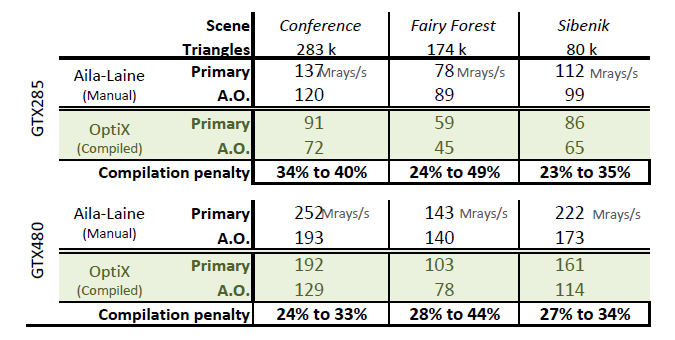
\includegraphics[width=0.5\linewidth]{fig7.png}}
\caption{Стоимость гибкости OptiX API и абстракции - a
сокращение производительности по сравнению с проблемно-ориентированным handoptimized трассировщиком лучей GPU [Эйла и Лэн 2009]. На наших сценах сравнительного теста этот штраф составляет приблизительно 25-35\% пикового Mrays/s со времени этой записи.}
\label{fig7}
\end{figure}
  механизм моделирует 4096 движущихся объектов, прослеживая лучи против статических 1.1 миллионов сцен многоугольника.
Механизм прослеживает 512 лучей зонда коллизии от каждого объектного центра, используя самую близкую программу хита и 40962/2 лучи угла обзора между всеми парами объектов, используя любую программу хита. Включая время, чтобы обработать результаты коллизии и выполнить объектную динамику, механизм достигает 25 миллионов лучей/секунда на GeForce GTX 280 и 48 миллионах
лучи в секунду на GTX 480. В то время как луч, бросая approch
не устойчиво ко всем операциям коллизии, это - часто используемый метод из-за своей простоты.
\subsection{результатов производительности}
Все результаты в этом разделе были представлены в HD 1080 пунктами ($1920\times1080$) разрешение. Чтобы оценить основную производительность, достижимую ядрами OptiX, мы воссоздали некоторые эксперименты, выполняемые в [Эйла и Лэн 2009] использование тех же сцен и позиций камеры. Мы сравненный наши сгенерированные ядра с этими вручную оптимизированными ядрами, чтобы измерить издержки, создаваемые уровнями абстракции программного обеспечения. Мы измеряли необработанную трассировку лучей и времена перекрестка, игнорируя времена для установки сцены, компиляции ядра, ускоряющих сборок структуры, буферных передач, и т.д. Эквивалентные ускоряющие структуры и рассчитывающие механизмы использовались в обеих системах. Таблица 1 показывает, что результаты для работают на NVIDIA GeForce GTX 285 и GeForceGTX 480 GPUs, усредненном по тем же 5 точкам зрения, используемым в исходной газете.
\begin{figure}[h!]
\center{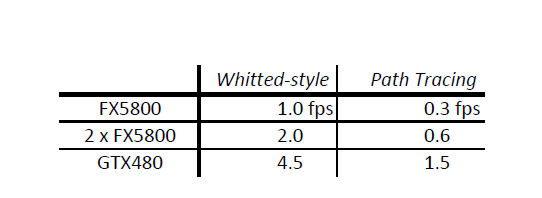
\includegraphics[width=0.5\linewidth]{fig8.png}}
\caption{Производительность приложения Гаража проекта в HD 1080 пунктов для 910 сцен спортивного автомобиля k-треугольника, на множестве конфигураций GPU. Частоты кадров включают трассировку лучей, штриховку и постобработку. Прослеженный результат пути показан в рисунке 1 (вершина).}
\label{fig8}
\end{figure}
  В то время как, как ожидалось, гибкость и программируемость OptiX дорого обходится, разрыв производительности все еще приемлем. Самый большой разрыв существует для окружающих лучей поглощения газов, который является частично
из-за остающегося недостатка в сравнительном тесте. В частности мы не выполняли сортировку луча и использовали более низкое число вторичных лучей за пиксель для наших измерений.
Таблица 2 показывает показатели производительности для Гаража Проекта (см. Раздел 8.2) на NVIDIA Quadro FX5800 и GeForce GTX 480 GPUs, который более показателен из реальной сцены, чем вышеупомянутый тест. Это приложение сложно по нескольким причинам. Во-первых, это - физический код трассировки пути с выборкой комплекса, многократными материалами и многими другими функциями. Это приводит к большому ядру, которое требует многих регистров, таким образом сокращая количество потоков, которые могут работать параллельно на GPU. Во-вторых, потоки более вероятно отличаться рано должный рассеяться или глянцевые легкие возвраты, которые приводят к различным материальным выполняемым программам построения теней, вызывая, уменьшало эффективность SIMT. В-третьих, подразделение геометрии сцены в многократные ускоряющие структуры (чтобы поддерживать анимацию) дополнительно увеличивает число операций для обхода луча по сравнению с монолитная структура данных. Тем не менее механизм OptiX может успешно объединить все эти различные программы и все еще сделать Гараж Проекта достаточно быстро, чтобы предложить интерактивную модификацию сцены и сходимости к фотореалистическому изображению в течение секунд.

Мы также сравнили реализацию OptiX-ISPM с опубликованной реализацией ЦП на компьютере Core 2 Quad Intel с рендерингом GTX485 GPU в разрешении HD 1080 пунктов. Мы оценили 20 сцен, включая “атриум Sponza” и “NS2” [Макгуайр и Луебк 2009]. Таблица 3 суммирует результаты производительности для четырех представительных сцен. Все были представлены с $4\times4$ подвыборка вглобальный сборочный шаг. Локальное время освещения включает буферы геометрии и схемы затенения. Время ввода-вывода измеряет передачу данных между OpenGL и ЦП или памятью CUDA. Сетевое время Локально + Глобальная переменная + Трассировка + ввод-вывод. Типичное ускорение было о $4\times$ для трассировки и $2.5\times$ в целом. “NS2” привел к самому низкому сетевому ускорению, с фотон OptiX прослеживает $3.0\times$ быстрее, чем ЦП один и сетевое время $1.8\times$ быстрее. Обратите внимание на то, что нахождение на той же стороне шины PCI так же важно как вычислительная производительность. Предотвращение передачи данных GPU ЦП может уменьшить время ввода-вывода на целых 50\%. Повышение эффективности обмена данными между двумя ПЧЕЛАМИ далее уменьшит стоимость этой передачи данных.
\subsection{ ограничений и будущая работа}
В настоящее время операции двойной точности поддержки во время выполнения OptiX в программах, но лучи сохранены в одинарной точности. Для некоторых приложений было бы желательно иметь луч двойной точности. Расширения буферного механизма OptiX подали бы некоторые проще заявки, такие как операции для добавляют, сокращения и сортирующие значения. 
\begin{figure}[h!]
\center{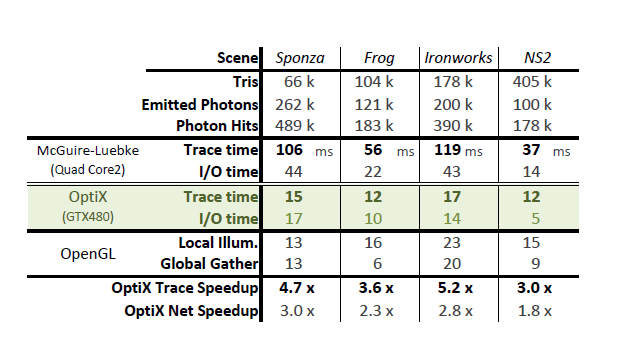
\includegraphics[width=0.5\linewidth]{fig9.png}}
\caption{Сравнение времени трассировки и передачи данных трассировщика OpenGL ray в разрешении HD 1080 пунктов для ЦП [Макгуайр и Луебк 2009] и реализации OptiX ISPM. У обоих есть то же локальное освещение, и глобальная переменная собирают времена. Трассировка фотона OptiX о 2.5 быстрее, чем ЦП один.}
\label{fig9}
\end{figure}
В некотором applicatons может также требоваться механизм динамического выделения памяти. Как с большинством компиляторов, есть бесконечные возможности для дополнительных оптимизационных проходов, которые будут добавлены, поскольку мы приобретаем опыт
с системой на важных приложениях. Кроме того, было бы интересно видеть, что дополнительные языки штриховки предназначаются для OptiX через PTX.
Ускоряющие структуры OptiX созданы, используя программу ограничивающего прямоугольника или специальный API, который поддерживает только треугольные данные. Чтобы создать лучшие ускоряющие структуры для программируемой геометрии, это было бы выгодно, чтобы обобщить ускоряющие сборки структуры, чтобы позволить
дополнительные программируемые операции. Это могло бы включать определяемое пользователем поле / примитивный тест перекрытия среди других операций. OptiX поддерживает несколько типов ускоряющих структур, но в настоящее время не предоставляет механизм пользователю, чтобы реализовать их собственное.
 \subsection{Заключений}
Система OptiX обеспечивает и высокоэффективный API трассировки лучей общего назначения. OptiX балансирует простоту использования с производительности, представляя простую модель программирования, на основе программируемого конвейера трассировки лучей для пользовательских программ единственного луча, которые могут быть скомпилированы в эффективное мегаядро самопланирования. Таким образом основа OptiX - JIT-компилятор, который обрабатывает программы,
отрывки определенного пользователями кода на языке PTX. OptiX связывает эти программы с узлами в графике, который определяет геометрическую конфигурацию и ускоряющие структуры данных, против которых прослежены лучи. Наши вклады включают низкоуровневый API трассировки лучей и связанную модель программирования, понятие программируемого
конвейер трассировки лучей и связанный набор программы типы, проблемно-ориентированный JIT-компилятор, который выполняет преобразования мегаядра и реализует несколько проблемно-ориентированной оптимизации и легкое представление сцены, которое предоставляет себя высокоэффективной трассировке лучей и поддержкам, но не ограничивает, структура графика сцены приложения. Механизм трассировки лучей OptiX - поставляющий продукт и уже поддерживает широкий диапазон
из приложений. Мы иллюстрируем широкую применимость OptiX с многократными примерами в пределах от упрощенного к довольно сложному. 
\subsection{Подтверждения}
Автомобиль, лягушка и модель механизма в рисунке 1 - любезность TurboSquid. Модель кролика 16 в цифрах и 4 является любезностью Stanford University Graphics Lab. Фил Миллер способствовал хранению усилия на ходу. Авторы ценят ценные комментарии от доктора Грега Хумфреиса и извлекли выгоду значительно из основы и многочисленных переговоров на трассировке лучей с элементами из Исследования NVIDIA и команды SceniX.
